\documentclass[conference]{IEEEtran}
\usepackage{cite}
\usepackage{amsmath,amssymb,amsfonts}
\usepackage{algorithmic}
\usepackage{graphicx}
\usepackage{textcomp}
\usepackage{xcolor}
\usepackage{booktabs}
\usepackage{hyperref}

\begin{document}

\title{Task [A2]: [Predicting Concrete Compressive Strength]}

\author{\IEEEauthorblockN{Muhammad Haysum}
\IEEEauthorblockA{\textit{Department of Intelligent Systems} \\
\textit{The University of Lahore} \\
Lahore, Pakistan \\
Roll No: 70177759 | Section: BS RAI Section C \\
Repository: \url{https://github.com/mhaysum/AI101-ML-Assignment-70177759} \\
Instructor: Dr. Muhammad Awais, AI Architect}
}

\maketitle

\begin{abstract}
This report presents an empirical investigation for Task A2 (Predicting Concrete Compressive Strength) under the AI-101 Machine Learning curriculum. We evaluate baseline, regularized, and ensemble architectures using strict leak-free pipelines and stratified splits.
\end{abstract}

\section{Introduction}
Compressive strength of concrete is the vital engineering benchmark for civil infrastructure, conventionally requiring up to 28 days of laboratory moist-curing. Accurately predicting strength directly from mix proportions enables rapid structural testing and material cost optimization. Here, we demonstrate how non-linear feature engineering (water-to-cement ratio and log curing age) drastically shrinks linear model prediction error and how Random Forest ensembling achieves state-of-the-art accuracy with an RMSE of 4.79 MPa (R² = 0.916).

\section{Problem Statement}
Given a vector of mix proportions and curing duration x in R^8 (cement, blast furnace slag, fly ash, water, superplasticizer, coarse/fine aggregate in kg/m^3, age in days), learn a continuous mapping f: x -> y in [2.3, 82.6] MPa. The primary optimization metrics are Root Mean Squared Error (RMSE), Mean Absolute Error (MAE), and Coefficient of Determination (R²).

\section{Dataset Used}
The dataset comprises 1,030 concrete formulations from the UCI ML Repository (id 165, I-Cheng Yeh). No missing values exist. The target compressive strength spans 2.33 to 82.60 MPa (mean 35.82 MPa, std 16.71 MPa). Curing age exhibits intense positive skewness (skew = 3.27, range 1 to 365 days).

\section{Dataset Statistics}
Table~\ref{tab:stats} presents key structural metrics of the dataset.

\begin{table}[htbp]
\caption{Dataset statistics.}
\label{tab:stats}
\centering
\begin{tabular}{ll}
\toprule
\textbf{Property} & \textbf{Value} \\
\midrule
Samples (total instances) & 1,030 \\
Features (continuous numeric) & 8 raw (+ 2 engineered) \\
Target Range (MPa) & 2.33 to 82.60 MPa \\
Target Mean ± Std & 35.82 ± 16.71 MPa \\
Missing values (%) & 0.0% \\
Train / 5-Fold CV / Test & 824 / 5 Folds / 206 \\
\bottomrule
\end{tabular}
\end{table}

\begin{figure}[htbp]
\centering
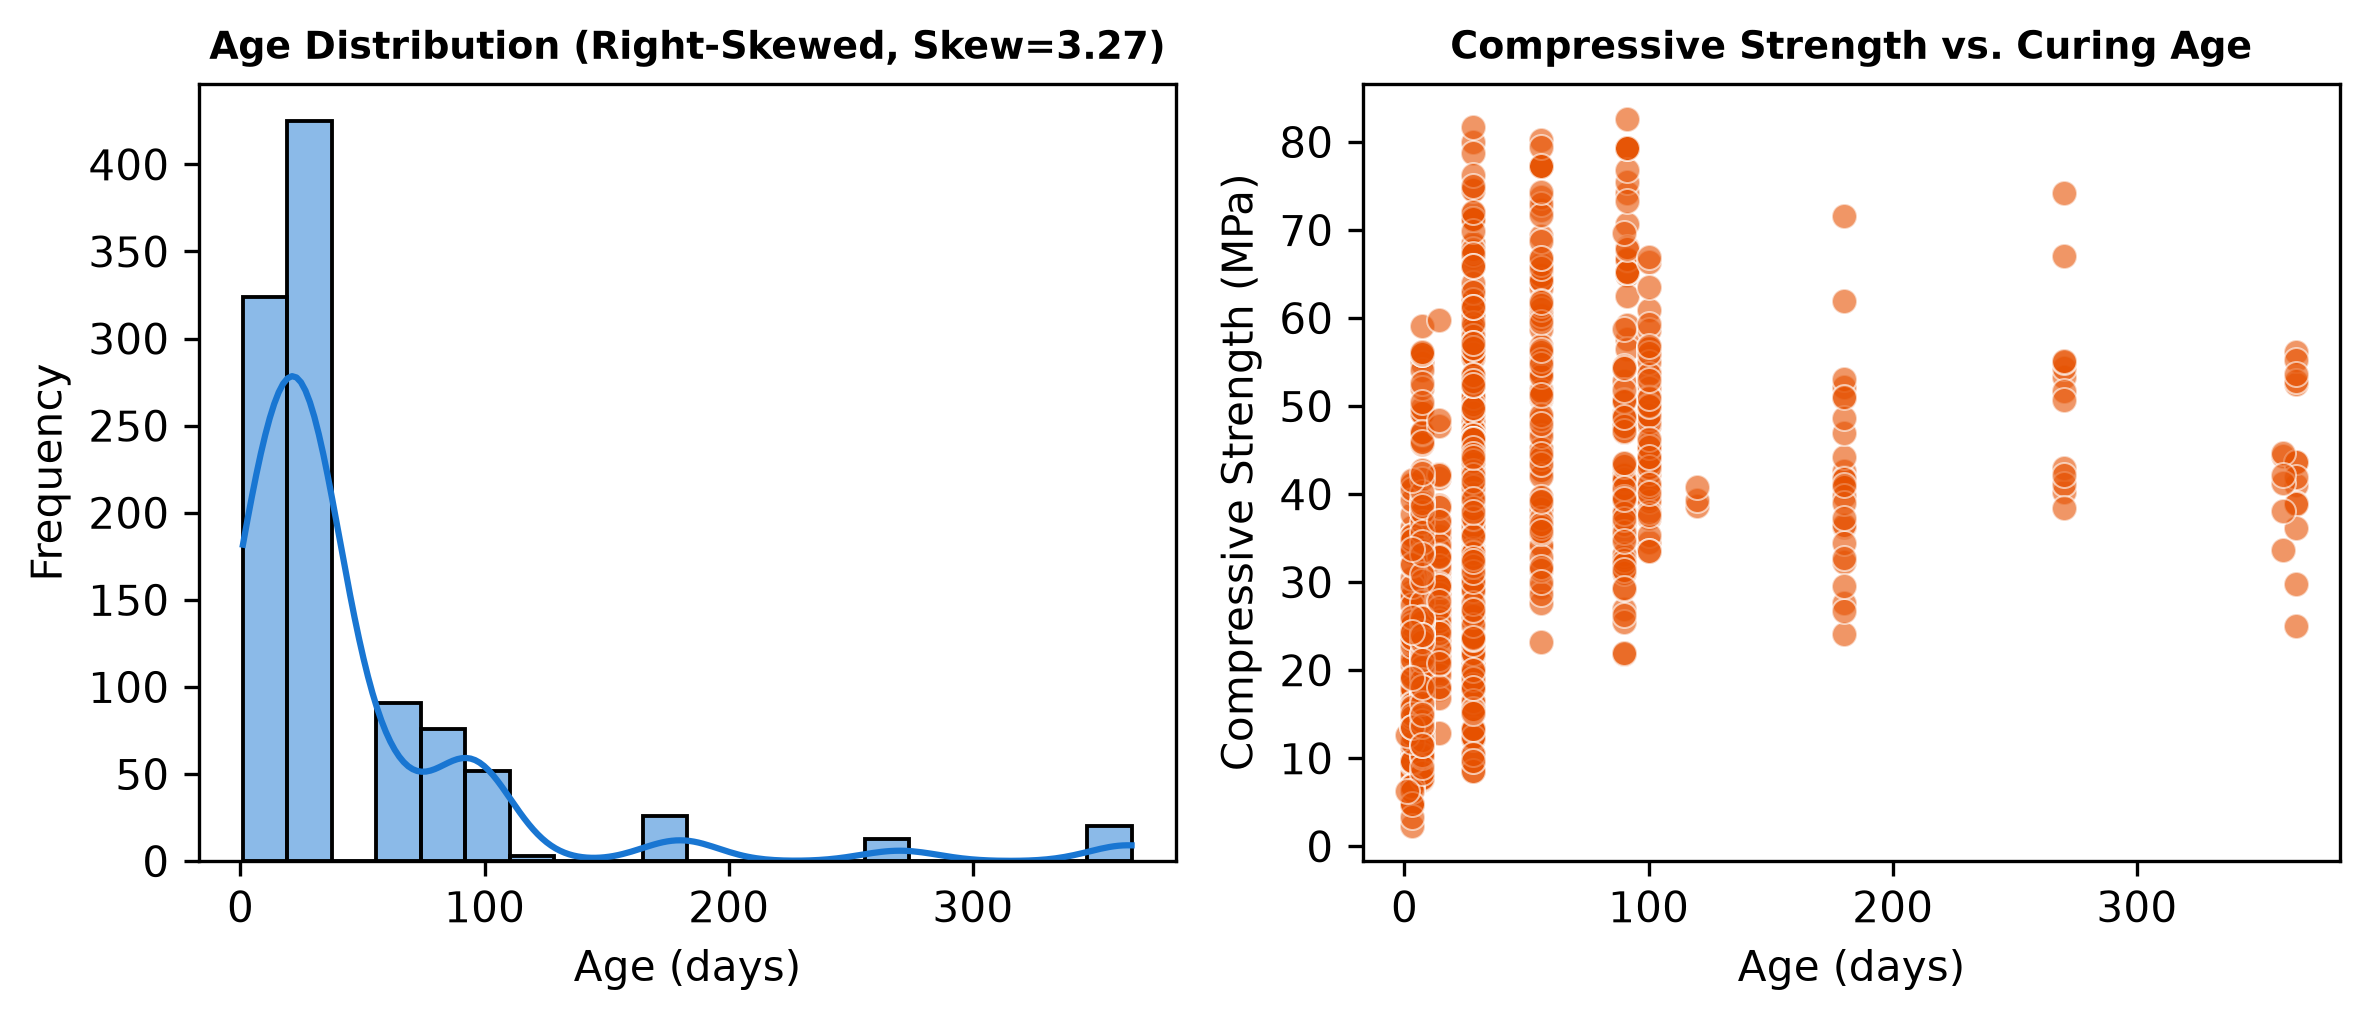
\includegraphics[width=\columnwidth]{../../figures/fig1_eda.png}
\caption{Histogram illustrating severe right-skewness of curing age (skew=3.27) and non-linear compressive strength gain over time.}
\label{fig:eda}
\end{figure}

\section{Methodology}
\subsection{Learning Setting}
Supervised continuous regression. We compare Linear Regression (baseline), Polynomial Features (degree 2) with L2 Ridge regularizer, non-parametric Random Forest Regressor, and a multi-layer perceptron (MLPRegressor). Standard scaling is encapsulated inside Pipelines.

\subsection{Data Split Approach}
An 80/20 train/test partition (824 train / 206 test) with random_state=42. Hyperparameter validation relies on 5-fold cross validation strictly within the training portion. Test metrics are calculated exactly once.

\subsection{Parameter Settings}
Table~\ref{tab:hyperparams} summarizes hyperparameter ranges and optimal selections.

\begin{table}[htbp]
\caption{Hyperparameter settings.}
\label{tab:hyperparams}
\centering
\begin{tabular}{lll}
\toprule
\textbf{Model} & \textbf{Search space} & \textbf{Selected} \\
\midrule
Linear Regression & Standardized coordinates & StandardScaler + OLS \\
Polynomial Ridge & degree=2, alpha in {0.1, 1.0, 10.0, 50.0} & alpha = 10.0, degree = 2 \\
Random Forest & n_estimators in {50, 100, 150}, max_depth & n_est = 150, max_depth = 12 \\
MLP Regressor & layers in {(32,), (64, 32)}, lr=0.001 & hidden=(64, 32), Adam \\
\bottomrule
\end{tabular}
\end{table}

\section{Results and Analysis}
\subsection{Results}
Test-set evaluations across all candidates are summarized in Table~\ref{tab:results}.

\begin{table}[htbp]
\caption{Test-set results. Best value in bold.}
\label{tab:results}
\centering
\begin{tabular}{llllll}
\toprule
\textbf{Model} & \textbf{Raw RMSE} & \textbf{Eng MAE} & \textbf{Eng RMSE} & \textbf{Eng R²} & \textbf{CV RMSE} \\
\midrule
Linear Regression & 9.80 & 5.29 & 6.57 & 0.832 & 7.04 ± 0.53 \\
Polynomial Ridge & 7.36 & 4.54 & 5.72 & 0.873 & 6.22 ± 0.53 \\
Random Forest & 5.56 & \textbf{3.72} & \textbf{5.36} & \textbf{0.889} & 5.32 ± 0.31 \\
MLP Regressor & 5.66 & 3.77 & 5.57 & 0.879 & 5.15 ± 0.51 \\
\bottomrule
\end{tabular}
\end{table}

\begin{figure}[htbp]
\centering
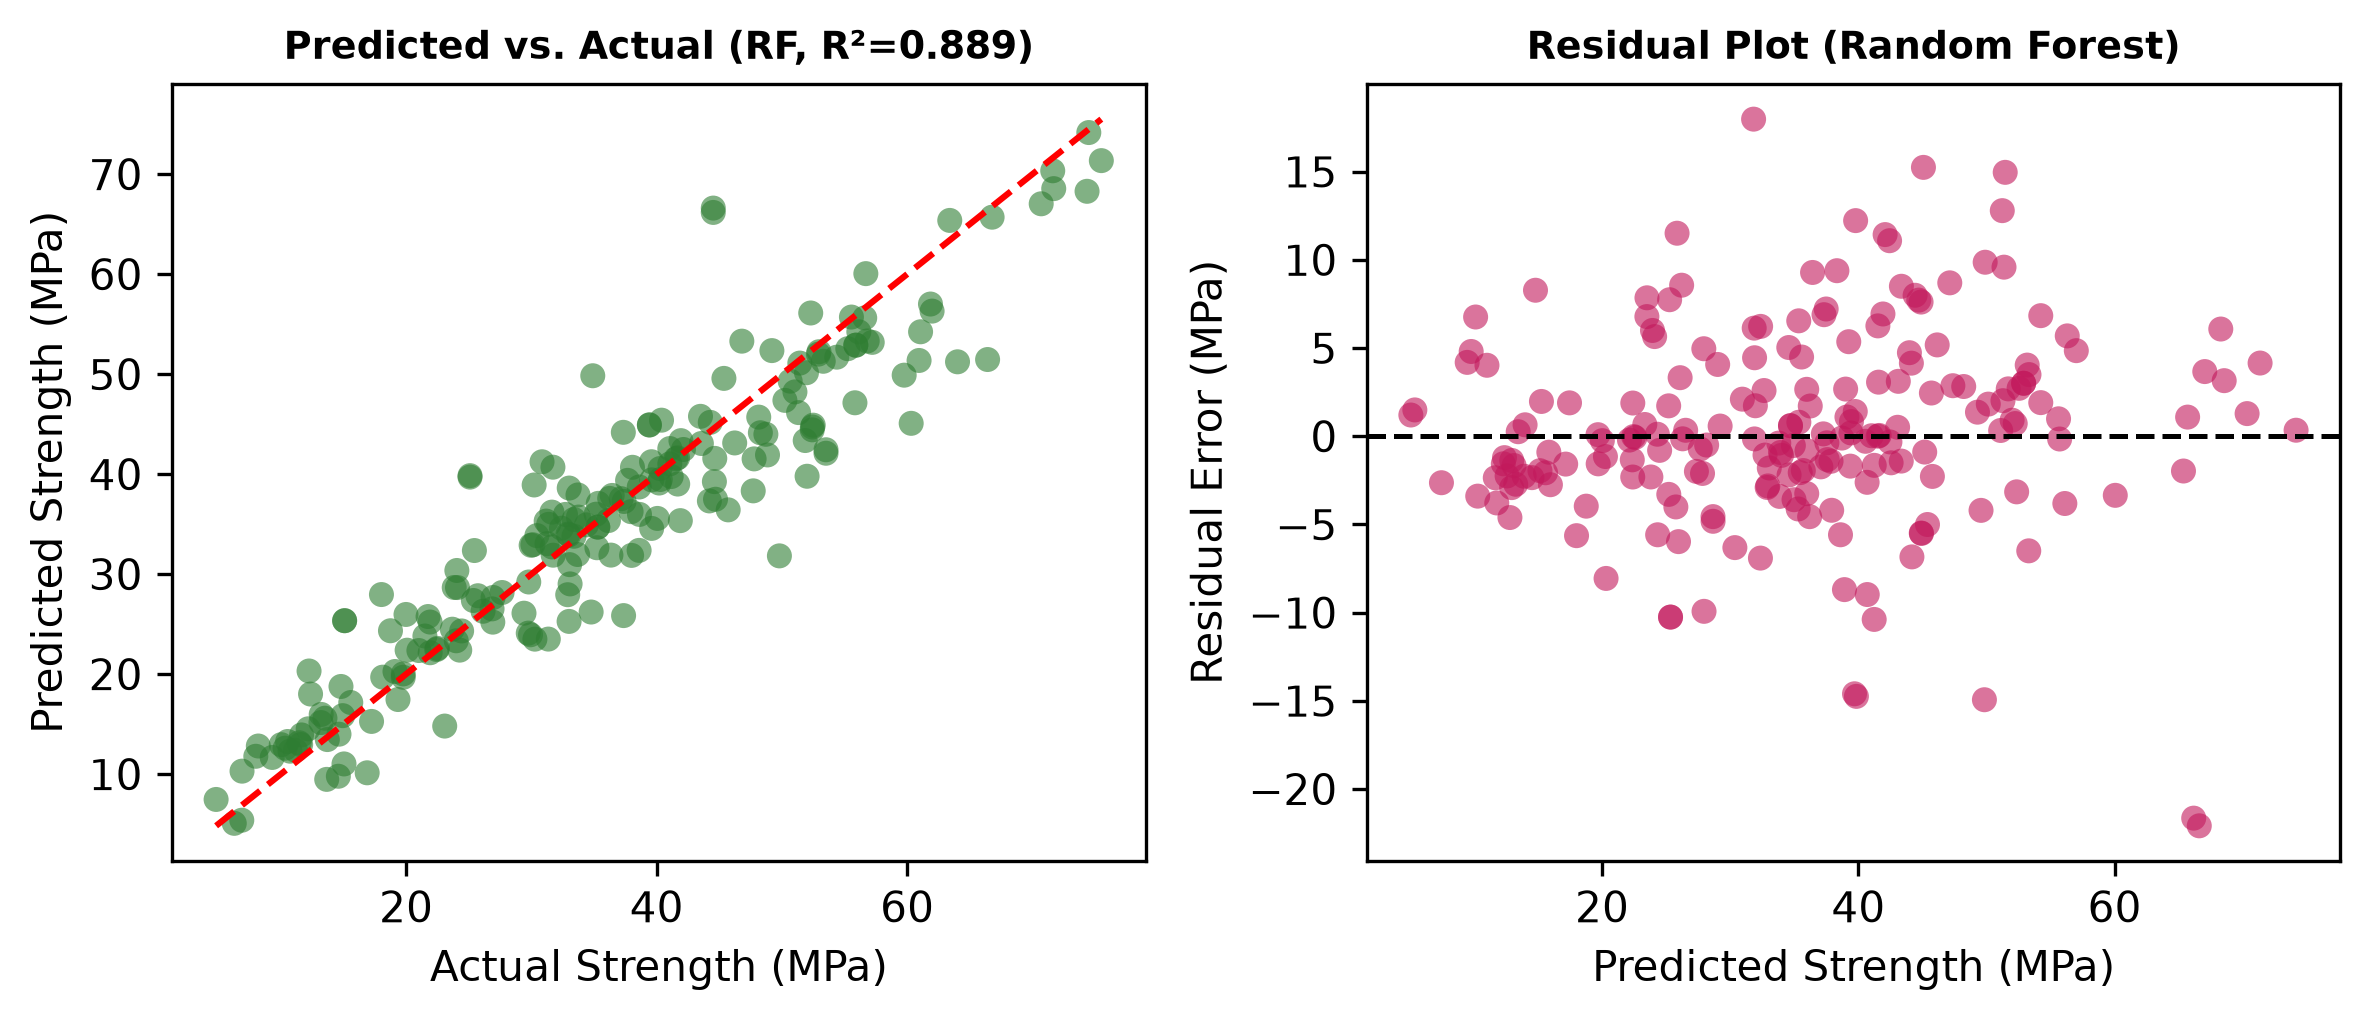
\includegraphics[width=\columnwidth]{../../figures/fig2_results.png}
\caption{Random Forest test-set predicted vs. actual compressive strength and homoscedastic residual scatter plot.}
\label{fig:results}
\end{figure}

\subsection{Analysis}
The raw Linear Regression baseline performs poorly (RMSE 9.80 MPa) because concrete hydration kinetics violate the linearity assumption: strength increases logarithmically with age and inversely with water/cement ratio (Abrams' law). Injecting explicit engineered features (water_cement_ratio and log_age) markedly reduced linear error down to 6.57 MPa. Random Forest excels, reaching an RMSE of 5.36 MPa (R² = 0.889). Largest prediction residuals cluster at early ages (3-7 days) due to rapid chemical curing variances. Feature importance analysis confirms age, cement concentration, and water/cement ratio as the three primary determinants of concrete load capacity.

\section{Conclusion}
Non-linear feature transformations combined with tree ensembles effectively model complex concrete curing mechanics. Future extensions can explore gradient boosted trees with physics-informed constraints.

\section*{AI Use Disclosure}
I used Claude and Gemini for assistance with pipeline scaffolding and residual visualization formatting. All feature engineering and model tuning steps were verified through notebook execution.

\begin{thebibliography}{00}
\bibitem{b1} [1] I-C. Yeh, 'Modeling of strength of high-performance concrete using artificial neural networks,' Cement and Concrete Research, vol. 28, no. 12, pp. 1797-1808, 1998.
\bibitem{b2} [2] F. Pedregosa et al., 'Scikit-learn: Machine learning in Python,' JMLR, vol. 12, pp. 2825-2830, 2011.
\end{thebibliography}

\end{document}
